\documentclass[13pt]{article}

\usepackage{adi}
\usepackage{enumitem}
\usepackage[disable]{todonotes}

\newcommand{\p}{\mathbf{p}}
\newcommand{\q}{\mathbf{q}}
\newcommand{\X}{\mathcal{X}}
\newcommand{\N}{\mathcal{N}}
\newcommand{\L}{\mathcal{L}}

\title{The principle of maximum entropy}
\author{\textsc{Adithya C. Ganesh}}

\begin{document}
\maketitle

\begin{abstract}
\noindent This expository paper covers the principle of maximum entropy, a key idea from information theory.  We will start by defining the Shannon entropy, which provides a measure of "disorder" or "expected surprise" of a random variable.  We will discuss the problem of prior distribution selection in statistics and build towards an analytic argument due to Wallis in 1962 that links maximizing entropy with statistical analysis.
\end{abstract}


\section{Introduction: what is entropy?}

Intuitively, the notion of entropy defines a measure of ``disorder'' or ``expected surprise'' given a probability distribution, as described by Claude Shannon in his seminal paper {\it A mathematical theory of communication \cite{shannon1948mathematical}}. This paper covers the principle of maximum entropy, an important tool with applications across various disciplines, including statistics, computer science, and physics.  

First, we will define the entropy over probability distributions and explore basic properties.  We will motivate the principle of maximum entropy and analyze the entropy of the Gaussian and exponential distributions.  Having established these preliminaries, we will discuss the general case of maximizing entropy over moment constraints.  Finally, we will discuss an analytic argument due to Wallis in 1962 that links maximizing entropy with statistical analysis.

As described by Shannon in \cite{shannon1948mathematical}, the entropy can be defined as follows. \\


\begin{definition}
  Let $X$ be a discrete random variable on a space $\mathcal{X}$ with probability mass function $\p(x)$.  We define the discrete (Shannon) entropy as follows, named after Boltzmann's H-theorem:
  \begin{align*}
    H(X) = \EE \left[ \log \frac{1}{\p(x)} \right] = \sum_{x \in \mathcal{X}} \p(x) \log \frac{1}{\p(x)}
  \end{align*}
\end{definition}


\begin{prop}
  The discrete entropy satisfies the following basic properties:
\begin{enumerate}[label=({\alph*})]
  \item $H(X) \geq 0$.
  \item $H(X) \leq \log |\mathcal{X}|$, with equality if and only if $X$ is distributed uniformly over $\mathcal{X}$.
\end{enumerate}
\end{prop}

\begin{proof}
  Part (a) follows from the fact that $\log \frac{1}{\p (x)} \geq 0$ for any $x \in \X$.  Hence the expectation is nonnegative and $H(X) \geq 0$.  
 
  To show part (b), we will apply Jensen's inequality (see the appendix for a formal statement).  First, note that $f(t) = \log (t)$ is concave.  Applying Jensen's inequality, we obtain:
  \begin{align*}
    \EE \left[ \log \frac{1}{\p (x)} \right] & \leq \log \EE \left[ \frac{1}{\p(x)} \right] \\
    &= \log \sum_{x \in \X} \p(x) \cdot \frac{1}{\p(x)} \\
    &= \log |\mathcal{X}|.
  \end{align*}
\end{proof}


A similar object to study is the so-called {\it relative entropy}, $D(\p || \q)$, which serves as a measure of distance between two probability distributions.  Importantly, $D(\p || \q) \neq D(\q || \p)$ in general, so the relative entropy is not a metric. \\

\begin{definition}
  Let $\p$ and $\q$ be probability distributions on a space $\mathcal{X}$.  Then the relative entropy\footnote{This quantity is also known as the Kullback-Leibler (KL) divergence and has numerous applications in statistics and physics.} $D(\p || \q)$ is defined as
  \begin{align*}
    D(\p || \q) = \EE_{x \sim \p(x)} \left[ \log \frac{\p(x)}{\q(x)} \right] = \sum_{x \in \mathcal{X}} \p(x) \log \frac{\p(x)}{\q(x)}.
  \end{align*}
\end{definition}

We will use the following basic fact in subsequent proofs: \\

\begin{lemma}
  The relative entropy is nonnegative.  That is, $D(\p || \q) \geq 0$ with equality if and only if $\p(x) = \q(x)$ for all $x \in \mathcal{X}$.
\end{lemma}

\begin{proof}
  Applying Jensen's inequality to the concave function $f(t) = \log(t)$, we obtain:
  \begin{align*}
    D(\p || \q) &= \EE_{x \sim \p(x)} \left[ \log \frac{\p(x)}{\q(x)} \right] \\
    &=  - \EE_{x \sim \p(x)} \left[ \log \frac{\q(x)}{\p(x)} \right] \\
    &\geq - \log \EE_{x \sim \p(x)} \left[ \frac{\q(x)}{\p(x)} \right] \\
    &= - \log \left( \sum_{x \in \mathcal{X}} \q(x) \right) \\
    &= \log 1 \\
    &= 0.
  \end{align*}

  Since $f(t)$ is strictly concave, equality can be achieved in Jensen's inequality only when $\frac{\q(x)}{\p(x)}$ is constant.  Since $\p$ and $\q$ are probability distributions, they must in fact be equal.
\end{proof}

We can define a version of the entropy for continuous random variables $X$. \\

\begin{definition}
\begin{align*}
  h(x) = \EE \left[ \log \frac{1}{\p(X)} \right] = \int_{-\infty}^{\infty} \p(x) \log \frac{1}{\p(x)}.
\end{align*}
\end{definition}

While these objects look similar, in fact the discrete and continuous definitions of entropy are rather different.  For instance, while $H(X) \geq 0$, in fact the differential entropy does not satisfy this property. \\

\begin{prop}
  The differential entropy of a Gaussian random variable $X \sim \N(0, \sigma^2)$ is $\log \sqrt{2 \pi e} \sigma$. \\
\end{prop}

\begin{proof} 
  Recall that the density function $p(x)$ is given by $p(x) = \frac{1}{\sqrt{2 \pi } \sigma} \exp \left( - \frac{x^2}{2 \sigma^2} \right)$.  Therefore
  \begin{align*}
    h(X) &= - \int_{-\infty}^{\infty} p(x) \log p(x) \, dx \\
    &= \int_{-\infty}^{\infty} p(x) \log \sqrt{2 \pi} \sigma \, dx + \int_{- \infty}^{\infty} p(x) \frac{x^2}{2 \sigma^2} \, dx \\
    &= \log \sqrt{2 \pi} \sigma + \frac{\sigma^2}{2 \sigma^2} \\
    &= \log \sqrt{2 \pi e} \sigma.
  \end{align*}
\end{proof}

\section{Prior probability distributions}

Suppose we have some prior knowledge about a phenomenon we would like to observe.  Given this knowledge, what is the best prior probability distribution?

The {\it principle of maximum entropy} states that we ought to choose the prior probability distribution that maximizes the entropy conditioned on our constraints.  In particular, this prior will be ``maximally disordered'' given the constraints; in a technical sense this prior makes the fewest assumptions.

There is significant debate on whether the principle of maximum entropy is the best choice for prior selection in statistics.  We do not concern ourselves here with these difficult issues, but we refer the interested reader to \cite{cover2012elements}\cite{jaynes1982rationale}\cite{mackay2003information}.

\section{Examples of maximum entropy}

We now present three simple examples of the maximum entropy principle.

\begin{theorem}
  Suppose $\mbf{p}$ is a discrete probability distribution on a finite set $\mathcal{X}$.  Then
  \begin{align*}
    H(\mbf{p}) \leq \log |\mathcal{X}|,
  \end{align*}
  with equality if and only if $\mbf{p}$ is uniform on $\mathcal{X}$.
\end{theorem}

This was proven in Section 1.  Intuitively, this states that with no constraints on a discrete probability distribution, the maximum entropy prior is uniform on the event space $\mathcal{X}$. \\

\begin{theorem}
  Let $\mbf{p}$ be a continuous probability distribution on $\mathbb{R}$ with variance $\sigma^2$.  Then
  \begin{align*}
    h(\p) \leq \log \sqrt{2 \pi e} \sigma.
  \end{align*}
  Equality holds if and only if $p$ is Gaussian with variance $\sigma^2$. \\
\end{theorem}

\begin{proof}
  We have already seen that the differential entropy of a Gaussian random variable  $G \sim \mathcal{N}(0, \sigma^2)$ is $h(G) = \log \sqrt{2 \pi e} \sigma$.

  Let $\p$ be a probability density on $\RR$ with variance $\sigma^2$ and mean $\mu$ (which exists by the definition of variance).  Let $\q$ be Gaussian with mean $\mu$ and variance $\sigma^2$.

  %\todo{Fix this issue with the means}

  \begin{lemma}
    Let $\p, \q$ be as defined above.  Then
    \begin{align*}
      \int_{-\infty}^{\infty} \q(x) \log \p(x) \, dx = \int_{-\infty}^{\infty} \p(x) \log \p(x) \, dx.
    \end{align*}
  \end{lemma}

  \begin{proof}
    Since $\p(x)$ is Gaussian, we can write down the density for $\log \p(x)$ easily.  Indeed,
    \begin{align*}
      \log \p(x) = - \log \sqrt{2 \pi \sigma^2} - \frac{x^2}{2 \sigma^2}.
    \end{align*}

    Now, to compute the integral, we can write
    \begin{align*}
      \int_{-\infty}^{\infty} \q(x) \log \p(x) &= - \log \sqrt{2 \pi \sigma^2} \int_{- \infty}^{\infty} \q(x) - \frac{1}{2 \sigma^2} \int_{-\infty}^{\infty} \q(x) x^2 \, dx \\
      &=- \log \sqrt{2 \pi \sigma^2} - \frac{\sigma^2}{2\sigma^2} \\
      &= - \log \sqrt{2 \pi e} \sigma,
    \end{align*}
    which agrees with a computation we did earlier.
  \end{proof}

  Now, applying this lemma, we can easily prove the main theorem:
  \begin{align*}
    0 & \leq D (\q || \p) = \int_{- \infty}^{\infty} \q(x) \log \frac{\q(x)}{\p(x)} \, dx \\
    & = - h(\q) - \int_{- \infty}^{\infty} \q(x) \log \p(x) \, dx \\
    & = - h(\q) - \int_{-\infty}^{\infty} \p(x) \log \p(x) \, dx \\
    &= -h(\q) + h(\p),
  \end{align*}
  so $h(\q) \leq h(\p)$ as claimed.
\end{proof}

\\

\begin{theorem}
  Let $\mbf{p}$ be a continuous probability density function on $(0, \infty)$ with mean $\mu$.  Then
  \begin{align*}
    h(p) \leq 1 + \log \mu,
  \end{align*}
  with equality if and only if $\mbf{p}$ is exponential with mean $\mu$.  That is, $p(x) = \frac{1}{\mu} \exp (- \frac{x}{\mu})$.
\end{theorem}

This theorem has a natural interprettion in physics.  Let $X$ be a random variable describing the height of molecules in the atmosphere.  The average potential energy of the molecules is fixed (mean $\lambda$), and the atmosphere tends to the distribution that has the maximum entropy.

\begin{proof}
  We will prove this result using Lagrange multipliers.  Let $\p$ be a probability distribution on $(0, \infty)$ with mean $\mu$.  Define
  \begin{align*}
    F(\p, \lambda_1, \lambda_2) &= - \int_{0}^{\infty} \p(x) \log \p(x) \, dx + \lambda_1 \left( \int_{0}^{\infty} \p(x) \, dx - 1 \right) + \lambda_2 \left( \int_{0}^{\infty} x \p(x) \, dx - \mu \right)  \\
    &= \int_{0}^{\infty} \mathcal{L}(x, \p(x), \lambda_1, \lambda_2) \, dx - \lambda_1 - \lambda_2 \mu,
  \end{align*}
  where $\mathcal{L}(x, \p, \lambda_1, \lambda_2) = - \p \log \p + \lambda_1 \p + \lambda_2 x \p$.  Taking partials,
  \begin{align*}
    \frac{\partial \mathcal{L}}{\partial \p} = - 1 - \log p + \lambda_1 + \lambda_2 x,
  \end{align*}
  and at a maximum entropy distribution we have $\frac{\partial \L}{\partial \p} = 0$, so that
  \begin{align*}
    \p(x) = \exp \left( \lambda_1 - 1 + \lambda_2 x \right),
  \end{align*}
  for $x \geq 0$.  
  
  Now, since $\int_{0}^{\infty} \p(x) \, dx$ is finite, we must have $\lambda_2 < 0$.  This implies
  \begin{align*}
    \int_{0}^{\infty} \p(x) &= 1 \\
    &= e^{\lambda_1 - 1} \int_{0}^{\infty} e^{\lambda_2 x} \, dx \\
    &= \frac{e^{\lambda_1 - 1}}{|\lambda_2|} \\
  \end{align*}
  so that $e^{\lambda_1 - 1} = |\lambda_2|$.  
  
  Now, since $\int_{0}^{\infty} x e^{\lambda_2 x} \, dx = \frac{1}{\lambda_2^2}$, the condition $\int_{0}^{\infty} x \, \p(x) \, dx = \mu$, so that $\lambda_2 = - \frac{1}{\mu}$.  
  
  Putting this together, we conclude  $\p(x) = \frac{1}{\mu} e^{-x / \mu}$, which is indeed the exponential distribution.
\end{proof}


\section{Generalizations}

Is it possible to obtain a maximum entropy solution under more general constraints?  

{\it Problem statement.} Maximize the entropy $h(f)$ over all probability densities $f$ satisfying the moment constraints below, where $S$ is the support set.
\begin{align*}
  \int_{S} f(x) r_i(x) dx = \alpha_i; \text{ for } 1 \leq i \leq m. \qquad \eqno(*)
\end{align*}

In particular, $f$ is a density on support set $S$ meeting moment constraints $\alpha_1, \alpha_2, \dots, \alpha_m$. \\

\begin{theorem}
  Let $f^{*}(x) = f_{\lambda}(x) = \exp (\lambda_0 + \sum_{i=1}^{m} \lambda_i r_i(x))$, $x \in S$, where $\lambda_0, \dots, \lambda_m$ are chosen so that $f^{*}$ satisfies the constraints in (*).  Then $f^{*}$ uniquely maximizes $h(f)$ over all probability densities $f$ that satisfy (*).
\end{theorem}

\begin{proof} (Sketch).

  We first sketch the argument for why the $\lambda_i$ can be chosen.  The constant $\lambda_0$ and the $n$ Lagrange multipliers $\lambda_1, \dots, \lambda_n$ solve the constrained optimization problem below:
  \begin{align*}
    \max_{\lambda_i} \left\{ \sum_{i=0}^{n} \lambda_i \alpha_i - \int_{S} \exp \left( \sum_{i=0}^{n} \lambda_i f_i(x) \right) \right\}.
  \end{align*}


  Under the Karush-Kuhn-Tucker (KKT) conditions, we can show that the optimization problem above has a unique solution, since the objective function is concave in the $\lambda_i$.  The full argument is out of the scope of this article, but we refer the interested reader to \cite{boyd2004convex}.

  Now, let $g$ satisfy the constraints in (*).  Then
  \begin{align*}
    h(g) &= - \int_{S} g \ln g \\
    &= - \int_{S} g \ln \frac{g}{f^{*}} f^{*} \\
    &= - \text{D} (g || f^{*}) - \int_{S} g \ln f^{*} \\
    &\leq - \int_{S} g \ln f^{*} \\
    &= - \int_{S} g \left( \lambda_0 + \sum_{i} \lambda_i r_i \right) \\
    &= - \int_{S} f^{*} \left( \lambda_0 + \sum_{i} \lambda_i r_i \right) \\
    &= - \int_{S} f^{*} \ln f^{*} \\
    &= h(f^{*})
  \end{align*}

  Note that equality holds in (a) if and only if $g(x) = f^{*}(x)$ for all $x$, which demonstrates uniqueness.
\end{proof}

\begin{example}[Boltzmann's dice \cite{cover2012elements}]
  Suppose that $n$ dice are rolled and the total number of spots is $n \alpha$.  What proportion of the dice are showing face $i$ where $i \in \left\{ 1, 2, \dots, 6 \right\}$?
\end{example}

We will count the number of ways that $n$ dice can fall so that $n_i$ dice show face $i$; this is just the multinomial coefficient $\binom{n}{n_1, n_2, \dots, n_6}$.

To find the most probable state, we will maximize the multinomial coefficient $\binom{n}{n_1, n_2, \dots, n_6}$ under the constraint $\sum_{i=1}^{6} i n_i = n \alpha$.

A form of Stirling's approximation states $n! \approx \left ( \frac{n}{e} \right )^{n}$.  In particular, this implies

\begin{align*}
  \binom{n}{n_1, n_2, \dots, n_6} & \approx \frac{\left ( \frac{n}{e} \right )^n}{\prod_{i=1}^{6} \left( \frac{n_i}{e} \right)^n} \\
  &= \prod_{i=1}^{6} \left( \frac{n}{n_i} \right)^{n_i} \\
  & = \exp \left( n H (\frac{n_1}{n}, \frac{n_2}{n}, \cdots, \frac{n_6}{n}) \right).
\end{align*}

This shows that maximizing $\binom{n}{n_1, n_2, \dots, n_6}$ under the given constraints is nearly equivalent to maximizing $H(p_1, \dots, p_6)$ under the constraint $\sum_{i} i p_i = \alpha$.  Applying the theorem, the maximum entropy distribution is

\begin{align*}
  p_i^{*} = \frac{e^{\lambda_i}}{\sum_{i=1}^{6} e^{\lambda_i}},
\end{align*}
where $\lambda$ is chosen so that $\sum_{i} i p_i^{*} = \alpha$.  Returning to the original question, the most probable state is $(np_1^{*}, np_2^{*}, \dots, n p_6^{*})$ and we expect $n_i^{*} = n p_i^{*}$ dice showing face $i$.


\section{The Wallis experiment}

This experiment is due to Graham Wallis who mentioned it to E.T. Jaynes in 1962 \cite{jaynes2003probability}.

Suppose Alice is a researcher trying to understand some data.  She is studying a phenomenon and wants to estimate a prior probability distribution among $m$ possible outcomes. She has some prior information about what the phenomenon looks like.  

To estimate the distribution, she runs the following experiment:

\begin{itemize}
  \item Randomly distribute $N$ quanta of probability, each worth $\frac{1}{N}$, among the $m$ possibilities.
  \item Check if the probability assignment is consistent with her prior information.  If inconsistent: reject and try again.
  \item If the assignment agrees with her prior information, her estimated prior distribution $\p$ is given by
    \begin{align*}
      \p_i = \frac{n_i}{N}; \qquad i \in \left\{ 1, 2, \dots, m \right\}
    \end{align*}
    where $\p_i$ is the probability of the $i$-th outcome, and $n_i$ is the number of quanta that were assigned to the $i$-th proposition.
\end{itemize}

As we'll see, this experiment has deep ties to the principle of maximum entropy.  We now ask: what is the most probable prior distribution Alice will arrive at?

The probability of any particular probability distribution $\p$ is given by a multinomial coefficient.
\begin{align*}
  \Pr(\mbf{p}) = \frac{N!}{n_1! n_2 ! \cdots n_m!} m^{-N},
\end{align*}

To find the most likely distribution $\p$, it suffices to maximize the term $A = \frac{N!}{n_1! n_2! \cdots n_m!}$, or a monotonically increasing function of $A$, e.g. $\frac{1}{N} \log A$.
\begin{align*}
  \argmax_{\mbf{p}} A  &= \argmax_{\mbf{p}} \frac{1}{N} \log A \\
  &= \argmax_{\mbf{p}} \frac{1}{N} \log \frac{N!}{n_1! n_2! \cdots n_m!} \\
  &= \argmax_{\mbf{p}} \frac{1}{N} \log \frac{N!}{(N \p_1)! (N \p_2)! \cdots (N \p_m)!} \\
  &= \argmax_{\mbf{p}} \frac{1}{N} \left( \log N! - \sum_{i=1}^{m} \log (N \p_i)! \right)
\end{align*}

What is the limit of this quantity as the number of trials $N \to \infty$?  Applying Stirling's approximation:
\begin{align*}
  \argmax_{\p} \lim_{N \to \infty} \left ( \frac{1}{N} \log A \right ) &= \argmax_{\p} \frac{1}{N} \left( N \log N - \sum_{i=1}^{m} N p_i \log (N p_i) \right) \\
  &= \argmax_{\p} \left ( \log N - \sum_{i=1}^{m} {p_i} \log (N p_i) \right ) \\
  & = \argmax_{\p} \left ( - \sum_{i=1}^{m} p_i \log p_i \right ) \\
  & = \argmax_{\p} H(\mbf{p}).
\end{align*}

In conclusion, Alice's experiment will most likely converge to the maximum entropy distribution as $N \to \infty$.


\section*{Appendix}

\begin{theorem}[Jensen's inequality] Let $X$ be a random variable, and let $\varphi$ be a convex function.  Then
  \begin{align*}
    \varphi(\EE [X]) \leq \EE \left[ \varphi(X) \right].
  \end{align*}
  If $\varphi$ is strictly convex, equality holds iff $X$ is uniformly distributed.
\end{theorem}

{\bf Graphical intuition.} The full proof is technical and out of the scope of this article.  The following picture describes the intuition behind this proof.

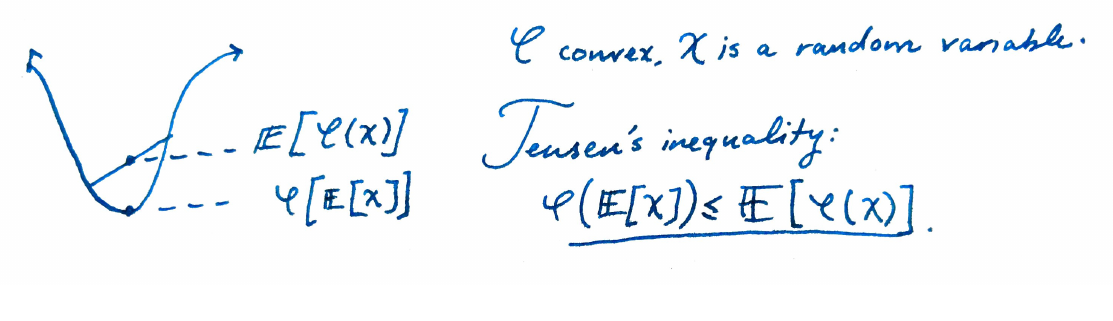
\includegraphics[width=\textwidth]{img/jensen}


\bibliographystyle{plain}
\nocite{*}
\bibliography{refs}

\end{document}
